% This should be \input first thing after \begin{document}


\pagestyle{titlepage}

\begin{center}
   {\Huge  \thedocsubtitle}  %Yes, I know title and subtitle are reversed!

  \vspace{5mm}

  {\Huge  \tdrtitle}  

  \vspace{10mm}

 {\LARGE \thedoctitle}

  \vspace{15mm}

\titleextra

  \vspace{10mm}
  \today
    \vspace{15mm}
    
\end{center}

\cleardoublepage

%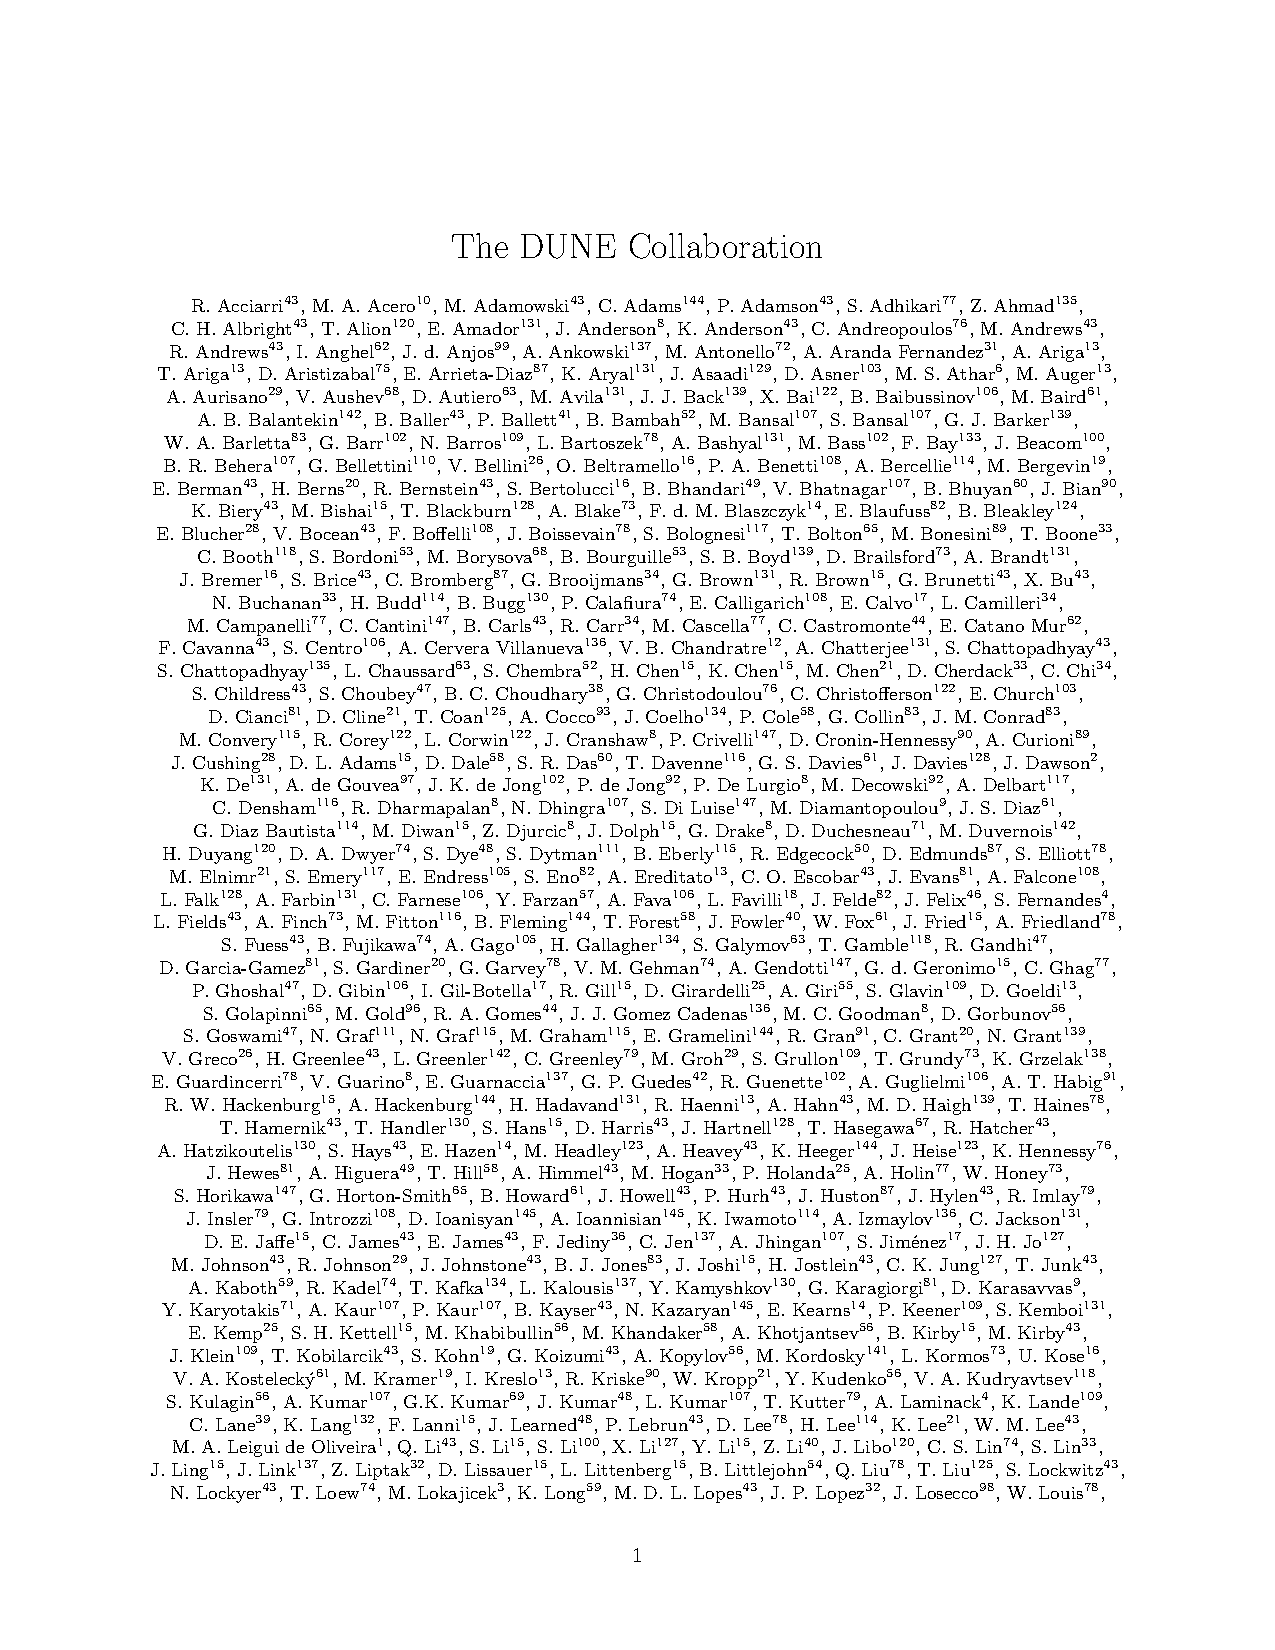
\includepdf[pages={-}]{tdr-authors.pdf}                        <--- add in later


\renewcommand{\familydefault}{\sfdefault}
\renewcommand{\thepage}{\roman{page}}
\setcounter{page}{0}

\pagestyle{plain} 

%\clearpage

\textsf{\tableofcontents}
%\clearpage


\textsf{\listoffigures}
%\clearpage

\textsf{\listoftables}
%\clearpage

%For acronym list to appear just after TOC, TOF, TOT
%\printnomenclature
%\clearpage

\iffinal\else
\textsf{\listoftodos}
\clearpage
\fi

\renewcommand{\thepage}{\arabic{page}}
\setcounter{page}{1}

\pagestyle{fancy}

% Set how header/footers look
\renewcommand{\chaptermark}[1]{%
\markboth{Chapter \thechapter:\ #1}{}}
\fancyhead{}
\fancyhead[RO,LE]{\textsf{\footnotesize \thechapter--\thepage}}
\fancyhead[LO,RE]{\textsf{\footnotesize \leftmark}}

\fancyfoot{}
\fancyfoot[RO]{\textsf{\footnotesize DUNE Technical Proposal}}
\fancyfoot[LO]{\textsf{\footnotesize \thedoctitle}}
\fancypagestyle{plain}{}

\renewcommand{\headrule}{\vspace{-4mm}\color[gray]{0.5}{\rule{\headwidth}{0.5pt}}}

% Not all main documents have any citations.
% When not built in "final" mode, add in one citation just to let the
% document build.
% If, after substantial editing a main document still lacks any
% citations then it should have its whole bibliography removed.
\ifdefined\isfinal\nocite{}\else\nocite{CD0}\fi



% see also preamble.tex
%%%%%%%%%%%%%%%%%%%%%%%%%% COMMON list for acronyms below %%%%%%%%%%%%%%%
\nomenclature{$\mathcal{O}(n)$}{of order $n$}
\nomenclature{3D}{3 dimensional (also 1D, 2D, etc.)} % not phys
\nomenclature{CDR}{Conceptual Design Report}
\nomenclature{CF}{Conventional Facilities}
\nomenclature{CP}{product of charge and parity transformations}
\nomenclature{CPT}{product of charge, parity and time-reversal transformations}
\nomenclature{CPV}{violation of charge and parity symmetry}
\nomenclature{DAQ}{data acquisition}
\nomenclature{DOE}{U.S. Department of Energy}
\nomenclature{DUNE}{Deep Underground Neutrino Experiment}
\nomenclature{ESH}{Environment, Safety and Health}
\nomenclature{eV}{electron-Volt, unit of energy (also keV, MeV, GeV, etc.)}
\nomenclature{FD}{far detector}
\nomenclature{FGT}{Fine-Grained Tracker}
\nomenclature{FSCF}{far site conventional facilities}
\nomenclature{NSCF}{near site conventional facilities}
\nomenclature{GUT}{grand unified theory}
\nomenclature{\ktyr}{exposure (without beam), expressed in kilotonnes times years}
\nomenclature{\ktMWyr}{exposure, expressed in kilotonnes $\times$ megawatts $\times$ years} 
\nomenclature{L}{level, indicates depth in feet underground at the far site, e.g., 4850L}
\nomenclature{LAr}{liquid argon}
\nomenclature{LArTPC}{liquid argon time-projection chamber}
\nomenclature{LBL}{long-baseline (physics)}
\nomenclature{LBNF}{Long-Baseline Neutrino Facility}
\nomenclature{MH}{mass hierarchy}
\nomenclature{MI}{Main Injector (at Fermilab)}
\nomenclature{ND}{near neutrino detector}
\nomenclature{NDS}{Near Detector Systems; refers to the collection of detector systems at the near site }
\nomenclature{near detector}{except in Volume 4 Chapter 7, this refers to the \textit{neutrino} detector system in the NDS}
\nomenclature{NND}{(used only in Volume 4 Chapter 7) near neutrino detector, same as ND}
\nomenclature{POT}{protons on target}
\nomenclature{QA}{quality assurance}
\nomenclature{SM}{Standard Model of particle physics}
\nomenclature{t}{metric ton, written \textit{tonne} (also kt)}
\nomenclature{TPC}{time-projection chamber (not used as `total project cost' in the CDR)}

%%%%%%%%%%%%%%%%%%%%%%%%% PROJECT VOLUME list for acronyms below %%%%%%%%%%%%%%%
\nomenclature{L1, L2, ...}{WBS level within the LBNF and DUNE Projects, where the overall Project is L1}
\nomenclature{MOU}{memorandum of understanding}
\nomenclature{SDSTA}{South Dakota Science and Technology Authority}
\nomenclature{WBS}{Work Breakdown Structure}


%%%%%%%%%%%%%%%%%%%%%%%%% PHYSICS VOLUME list for acronyms below %%%%%%%%%%%%%%%
\nomenclature{BR}{branching ratio}
\nomenclature{DM}{dark matter}
\nomenclature{DSNB}{Diffuse Supernova Neutrino Background}
\nomenclature{GLoBES}{General Long-Baseline Experiment Simulator (software package)}
\nomenclature{L/E}{length-to-energy ratio}
\nomenclature{LRI}{long-range interactions}
\nomenclature{$M_{\odot}$}{solar mass}
\nomenclature{NC}{neutral current (interaction)}
\nomenclature{NH}{normal (mass) hierarchy}
\nomenclature{NSI}{nonstandard interactions}
\nomenclature{MSW}{Mikheyev-Smirnov-Wolfenstein (effect)}
\nomenclature{SME}{Standard-Model Extension}
\nomenclature{SUSY}{supersymmetry}
\nomenclature{WIMP}{weakly-interacting massive particle}

%%%%%%%%%%%%% PROJECT AND PHYSICS VOLUME list for acronyms below %%%%%%%%%%%%
\nomenclature{C.L.}{confidence level}

%%%%%%%%%%%%% PROJECT AND DETECTORS VOLUME list for acronyms below %%%%%%%%%%%%

\nomenclature{APA}{anode plane assembly} 
\nomenclature{BLM}{(in Volume 4) beamline measurement (system); (in Volume 3) beam loss monitor}
\nomenclature{CPA}{cathode plane assembly}
\nomenclature{ECAL}{electromagnetic calorimeter}
\nomenclature{GAr}{gaseous argon}
\nomenclature{HV}{high voltage}

%%%%%%%%%%%%% PHYSICS AND DETECTORS VOLUME list for acronyms below %%%%%%%%%%%%
\nomenclature{CC}{charged current (interaction)}
\nomenclature{DIS}{deep inelastic scattering}
\nomenclature{FSI}{final-state interactions}
\nomenclature{GEANT4}{GEometry ANd Tracking, a platform for the simulation of the passage of particles through matter using Monte Carlo methods} 
\nomenclature{GENIE}{Generates Events for Neutrino Interaction Experiments (an object-oriented neutrino Monte Carlo generator)} 
\nomenclature{MC}{Monte Carlo (detector simulation methods)}
\nomenclature{QE}{quasi-elastic (interaction)}

%%%%%%%%%%%%%%%%%%%%%%%%% DETECTORS VOLUME list for acronyms below %%%%%%%%%%%%%%%

\nomenclature{CE}{Cold Electronics}
\nomenclature{COB}{cluster on-board (motherboards)} %?
\nomenclature{CRP}{Charge-Readout Planes }
\nomenclature{DRAM}{dynamic random access memory}
\nomenclature{FE}{front end (electronics)}
%\nomenclature{Fermilab (also FNAL)}{Fermi National Accelerator Laboratory (in Batavia, IL, the Near Site)}
%\nomenclature{FNAL}{see Fermilab}
\nomenclature{FPGA}{field programmable gate array} %?
\nomenclature{FGT}{Fine-Grained Tracker}
\nomenclature{FS}{full stream (data volumes)} %?
\nomenclature{LEM}{Large Electron Multiplier}
%\nomenclature{LNGS}{Laboratori Nazionali (National Laboratory) del Gran Sasso (in L'Aquila, Italy)}
%\nomenclature{MaVaNs}{mass varying neutrinos}
\nomenclature{MIP}{minimum ionizing particle}
\nomenclature{MTS}{Materials Test Stand}
\nomenclature{MuID}{muon identifier (detector)}
%\nomenclature{OPERA}{Oscillation Project with Emulsion-Racking Apparatus (experiment at LNGS)}
\nomenclature{octant}{any of the eight parts into which 4$\pi$ is divided by three mutually perpendicular axes}
%\nomenclature{OD}{outer diameter}
\nomenclature{PD}{photon detection (system)}
\nomenclature{PMT}{photomultiplier tube}
\nomenclature{RCE}{reconfigurable computing element}
\nomenclature{RIO}{reconfigurable input output}
\nomenclature{RPC}{resistive plate chamber}
\nomenclature{SiPM}{silicon photomultiplier}
\nomenclature{S/N}{signal-to-noise (ratio)}
\nomenclature{SSP}{SiPM signal processor}
\nomenclature{STT}{straw tube tracker}
%\nomenclature{SURF (also Sanford Lab)}{Sanford Underground Research Facility (in Lead, SD, the Far Site)}
\nomenclature{TR}{transition radiation}
%\nomenclature{W}{Watt (also mW, kW, MW) }
%\nomenclature{WA105}{Single-Phase LArTPC and the Long Baseline Neutrino Observatory Demonstration}
\nomenclature{WLS}{wavelength shifting}
\nomenclature{ZS}{zero suppression}

\fixme{Do we need GVKM, SNO, QCD,  PANDORA,  aTCA and microTCA, AMC, MCH, CPU, GPU, VHDL, OpenCL, PTP, Sync-E, GPS, IEEE, WR}





